
%---- Begin PDF metadata ---------%
\usepackage{hyperref}
\hypersetup{%
	pdftitle={URDAD as Quality-Driven Process},%
	pdfauthor={Fritz Solms, Stefan Gruner and Cuen Edwards},%
	pdfsubject={},%
	pdfkeywords={URDAD, Quality driver}%
}
%---- End PDF metadata ---------%

% --- Graphics support ----%
\usepackage{graphicx}

% ---- Ticking clock for presentation ---%
% Duration of presentation = 20 minutes, change color at 50% and 80% of time, update clock every 29 seconds
% This is used in conjunction with \tdtime, \crono or \cronominutes
\usepackage[font=Times,timeinterval=29, timeduration=20.0, timedeath=0, fillcolorwarningsecond=white!60!yellow,timewarningfirst=50,timewarningsecond=80]{tdclock}


%--------------- Begin Beamer styling  -------------%

\usetheme{Berkeley}
% default 
%	AnnArbor | Antibes | Bergen |
%	Berkeley | Berlin | Boadilla |
%	boxes | CambridgeUS | Copenhagen |
%	Darmstadt | default | Dresden |
%	Frankfurt | Goettingen |Hannover |
%	Ilmenau | JuanLesPins | Luebeck |
%	Madrid | Malmoe | Marburg |
%	Montpellier | PaloAlto | Pittsburgh |
%	Rochester | Singapore | Szeged |
%	Warsaw

\setbeamertemplate{background canvas}{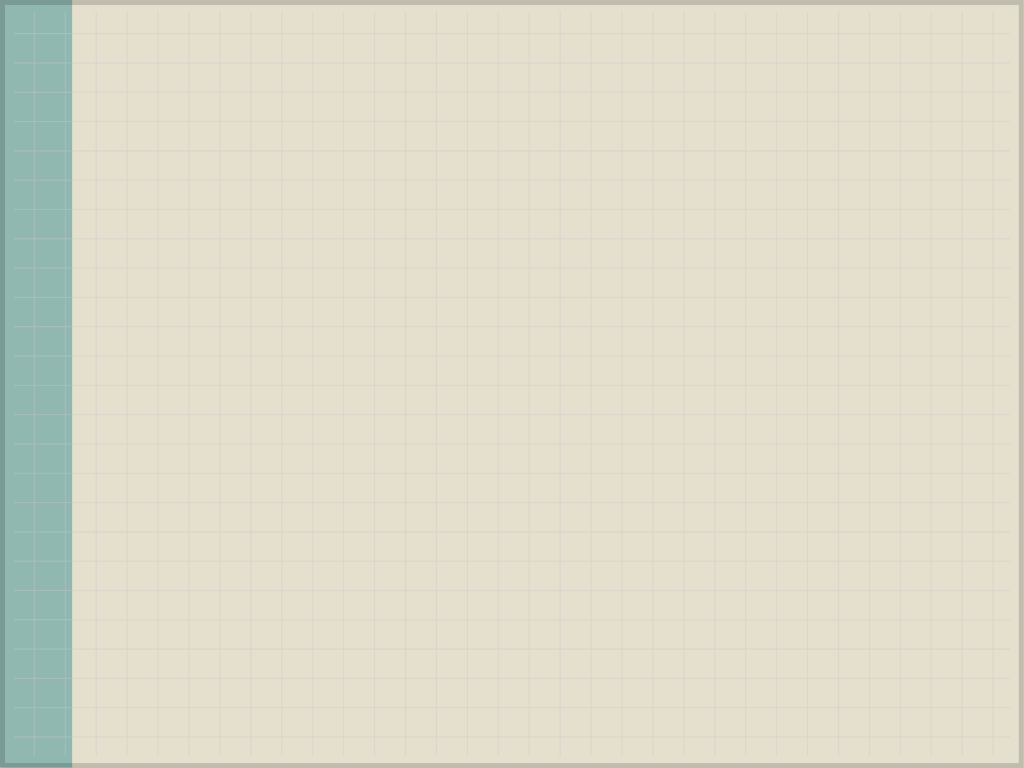
\includegraphics
	[width=\paperwidth,height=\paperheight]{background.png}}
\setbeamercolor{structure}{fg=DarkSlateGray} 
\setbeamercolor{normal text}{fg=Black} 
%\setbeamercolor{alerted text}{fg=Crimson} 
%\setbeamercolor{alerted text}{fg=DarkRed} 
\setbeamerfont{structure}{series=\bfseries} 
%\setbeamersize{text margin left=10mm}

% To insert outline slides before every section
%\AtBeginSection[]
%{
%   \begin{frame}
%       \frametitle{Outline}
%       \tableofcontents[currentsection]
%   \end{frame}
%}

%--------------- Begin Beamer styling  -------------%

%--- Begin Code listing suport for URDAD DSL --------%
\usepackage{listings}
\lstdefinelanguage{urdad}
{
keywords=
  {Model,ResponsibilityDomain,Query,Constraint,QualityConstraint,FunctionalRequirements,receiving,yielding,
  StateConstraint,stateAssessmentProcess,InverseConstraint,inverseOf,AndConstraint,AND,OrConstraint,OR,
  XorConstraint,XOR,from,to,many,BasicDataType,DataStructure,is,abstract,has,Variable,ofType,Constant,
  ValueOf,Exception,attribute,identification,identifying,association,linking,aggregate,component,
  QualityRequirement,requiredBy,constraint,with,constructedUsing,ResultConstraint,PreCondition,
  raises,checks,PostCondition,ensures,use,toAddress,if,ServiceContract,undoneUsing,Request,Result,
  Service,realizes,doSequential,choice,else,doConcurrent,blocking,Concurrency,wait,until,create,set,
  equalTo,add,remove,requestService,on,raiseException,returnResult,while,do,forAll,Note},%
sensitive=true,%
alsoletter={\$},%
comment=[l]{\#},%
string=[b]",%
string=[b]'%
}

%\definecolor{OliveGreen}{cmyk}{0.64,0,0.95,0.40}
%\definecolor{CadetBlue}{cmyk}{0.62,0.57,0.23,0}
\definecolor{lightgray}{gray}{0.9}
\lstset{
language=urdad,  
basicstyle=\ttfamily\tiny,
keywordstyle=\itshape\color{blue},
%keywordstyle=\color{blue},        % Keywords font ('*' = uppercase)
commentstyle=\color{gray},           
numbers=left,                           % Line nums position
numberstyle=\tiny,                      % Line-numbers fonts
stepnumber=1,                           % Step between two line-numbers
numbersep=5pt,                          % How far are line-numbers from code
backgroundcolor=\color{lightgray}, % Choose background color
frame=none,                             % A frame around the code
tabsize=2,                              % Default tab size
captionpos=b,                           % Caption-position = bottom
breaklines=true,                        % Automatic line breaking?
breakatwhitespace=false,                % Automatic breaks only at whitespace?
showspaces=false,                       % Dont make spaces visible
showtabs=false,                         % Dont make tabls visible
columns=flexible,                       % Column format
%morekeywords={__global__, __device__},  % CUDA specific keywords
}

